\documentclass[tikz,border=3pt]{standalone}
\usepackage[T1]{fontenc}
\usepackage{helvet}
\renewcommand{\familydefault}{\sfdefault}
\usepackage{setspace}
\usetikzlibrary{positioning,arrows.meta,shapes.geometric}

\begin{document}
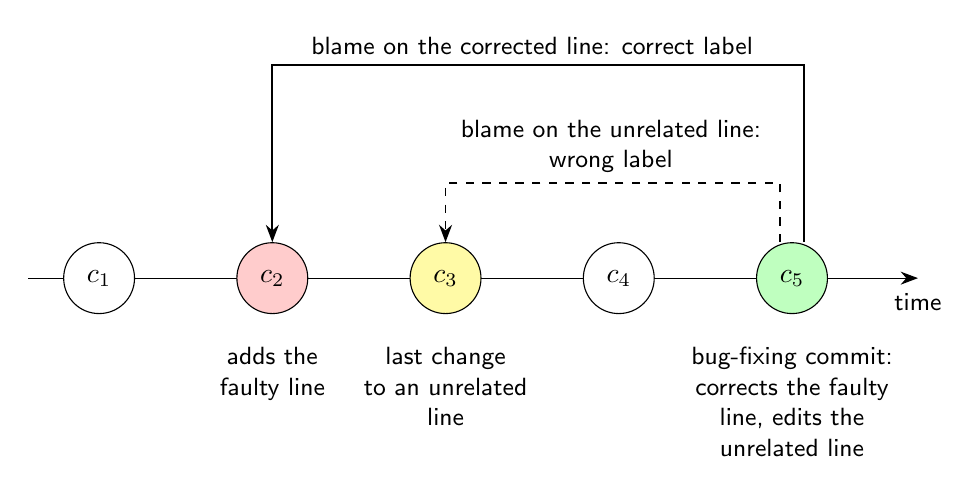
\begin{tikzpicture}[
  c/.style={circle, draw, minimum size=9mm, inner sep=0pt},
  note/.style={align=center, font=\small, text width=27mm},
  arr/.style={-{Stealth[length=2.2mm]}, semithick}]
\draw[-{Stealth[length=2.2mm]}] (0,0) -- (11.3,0) node[below=2pt, font=\small] {time};
\node[c, fill=white] (c1) at (0.9,0) {$c_1$};
\node[c, fill=red!20] (c2) at (3.1,0) {$c_2$};
\node[c, fill=yellow!35] (c3) at (5.3,0) {$c_3$};
\node[c, fill=white] (c4) at (7.5,0) {$c_4$};
\node[c, fill=green!25] (c5) at (9.7,0) {$c_5$};
\node[note, below=3mm of c2] {adds the\\faulty line};
\node[note, below=3mm of c3] {last change\\to an unrelated\\line};
\node[note, below=3mm of c5] {bug-fixing commit:\\corrects the faulty\\line, edits the\\unrelated line};
\draw[arr] ([xshift=1.5mm]c5.north) -- ++(0,2.25) -| (c2.north);
\node[font=\small, anchor=south] at (6.4,2.72) {blame on the corrected line: correct label};
\draw[arr, dashed] ([xshift=-1.5mm]c5.north) -- ++(0,0.75) -| (c3.north);
\node[font=\small, anchor=south, align=center] at (7.4,1.22) {blame on the unrelated line:\\wrong label};
\end{tikzpicture}
\end{document}
